\documentclass[../rapport.tex]{subfiles}
\graphicspath{{\subfix{ressources/}}}


\begin{document}
\subsection{Base de données}
	
	\paragraph{Choix du système de gestion de base de données :}
		Lors de la création et de l'implémentation de la base de données il a fallu dans un
		premier temps établir le système de base de données qui serait utilisé. 
		Il a été décidé au sein du groupe que ce serait MariaDB qui serait utilisé suite
		à notre expérience avce ce dernier lors du cours de Base de données I au premier
		quadrimestre.
	
	\bigskip 
	
	\paragraph{Stratégie d'implémentation : }
		La stratégie choisie quant à l'implémentation de la base de données a été de se baser
		sur le diagramme construit lors de la phase de modélisation au premier quadrimestre.
		Le but était de construire table par table la base de données tout en testant à chaque
		fois les relations entre celles-ci afin de répérer d'éventuels omissions qui auraient été
		commises lors de la rédaction du rapport de modélisation.

		\medskip

		C'est pourquoi, notre base de données a subit une légère refonte au cours de cette phase
		d'implémentation, afin de s'adapter au mieux à l'usage que nous allions en faire. Un 
		nouveau diagramme d'entité relation a été réalisé afin de voir plus clairement les 
		modifications effectuées.

		\medskip
		
		Par la suite nous avons conservé cette base de données comme modèle pour utiliser le 
		Data Acces Layer : Spring Data JPA. Qui permet d'établir la communication entre la
		base de données MariaDB et l'API en auto générant cette base de donnée sur base de 
		classes de type @Entity créées dans le code de l'API.
		
	\bigskip

	\paragraph{Data Acces Layer : }
	Pour le Data Access Layer nous avons décidé de nous servir de celui proposé par le framework
	Spring utlisé pour l'implémentation de l'API : Spring Data JPA.

	\medskip

	Data JPA nous a permis de générer une seconde base de données de manière automatisée au 
	travers de classes de type \@Entity. Ces classes permettent de gérer de manière orientée
	objet les différentes entités présentes dans la base de données mais également de les 
	mettre en relation en définissant des foreign key.

	\medskip

	Data JPA met également à disposition un jeu d'interfaces appelés repositories qui 
	définissent des méthodes de type \"requêtes\" afin d'établir une connexion aisée avec 
	la base de données.

	\medskip

	L'utilisation de ce Data Acces Layer nous a permis de simplifier l'implémentation de
	la base de données ainsi que sa mise en relation avec l'API. Cela nous a également 
	apportés quelques notions de bases du principe d'API qui nous semblaient encore floues.
	Toutefois, bien que ce framework nous ai été utile au départ il a été sources de problèmes
	lors de la suite de l'implémentation de l'API.

	\bigskip

	\paragraph{Problèmes rencontrés avec le Data Acces Layer :}
	Nous avons rencontrés 3 problèmes majeurs avec DATA JPA au cours de l'implémentation.
	
	\medskip

	\begin{enumerate}
		\item\textbf{Foreign Key :} Des problèmes ont été rencontrés avec les définitions des
			foreign keys. En effet celles ci sont définies via des instances d'objets 
			correspondants aux entités vers lesquelles elles font référence. Cela a engendré 
			des problèmes de cast au niveau des types de données insérés/récupérés dans la BDD.
			Pour faire face à ces problèmes nous avons décidé d'implémnter directement dans la
			BDD les foreign key posant problème. Ce qui explique toutes les foreign key ne soient
			pas représentées dans Spring.
		\medskip
		\item\textbf{Composite Primary Key :} Des problèmes avec des composites primary key 
			ont été rencontré lorsqu'un des membres de cette primary key était une foreign key 
			d'une autre table. En guise de résolution nous avons procédé comme au point précédent.
		\medskip
		\item\textbf{Test unitaires :} Le membre du groupe en charge des tests unitaires n'ayant
			pas fait les test unitaires liés à l'API c'est le membre du groupe en charge de l'API
			et de la BDD qui a du reprendre la tâche. 
			La base de données et l'API étant déjà presque terminées il était trop tard pour 
			pouvoir trouver une solution à ce problème. 
			En effet, c'est le framework DATA JPA qui s'occupe de la génération de la BDD ainsi 
			que des reqûetes qui sont liées à cette génération. Pour le testing de la BDD, une 
			nouvelle BDD en mémoire (Base de données H2) doit être utilisée afin de tester DATA
			JPA, or nous avons du faire face à un problème de communication entre les 2 modules 
			du framework sans pouvoir y trouver de solution. Ce qui explique la presque absence 
			de tests unitaires pour cette partie. Toutefois, comme expliqué dans la stratégie 
			d'implémentation la base de données a été testée au fur et à mesure de son 
			implémentation.
	\end{enumerate}

	\bigskip

	\paragraph{Points forts de la base de données :}
	La base de données a été pensée de manière à faciler l'ajout des différentes extensions.
	Bien que la seule extension présente dans la BDD soit celle des assurances.
	\medskip

	En effet, grâce à la table \textbf{CASH\_BALANCES} l'ajout de l'extension permettant de gérer
	des comptes multi-devises est facilité car les comptes admettent déjà des mutliples balances
	permettant ainsi au compte de posséder plusieurs devises.

	\medskip

	Pour ce qui de l'extension concernant la gestion des fraudes une table contenant l'historique
	des transactions \textbf{TRX\_HISTORY} a déjà été mise en place afin de permettre de controller
	les virements par leur date, l'envoyeur et le réceptionneur. 
	
	
	\newpage
	\subsection{Diagramme d'entité relation}
	
		\begin{figure}[h]
			\centering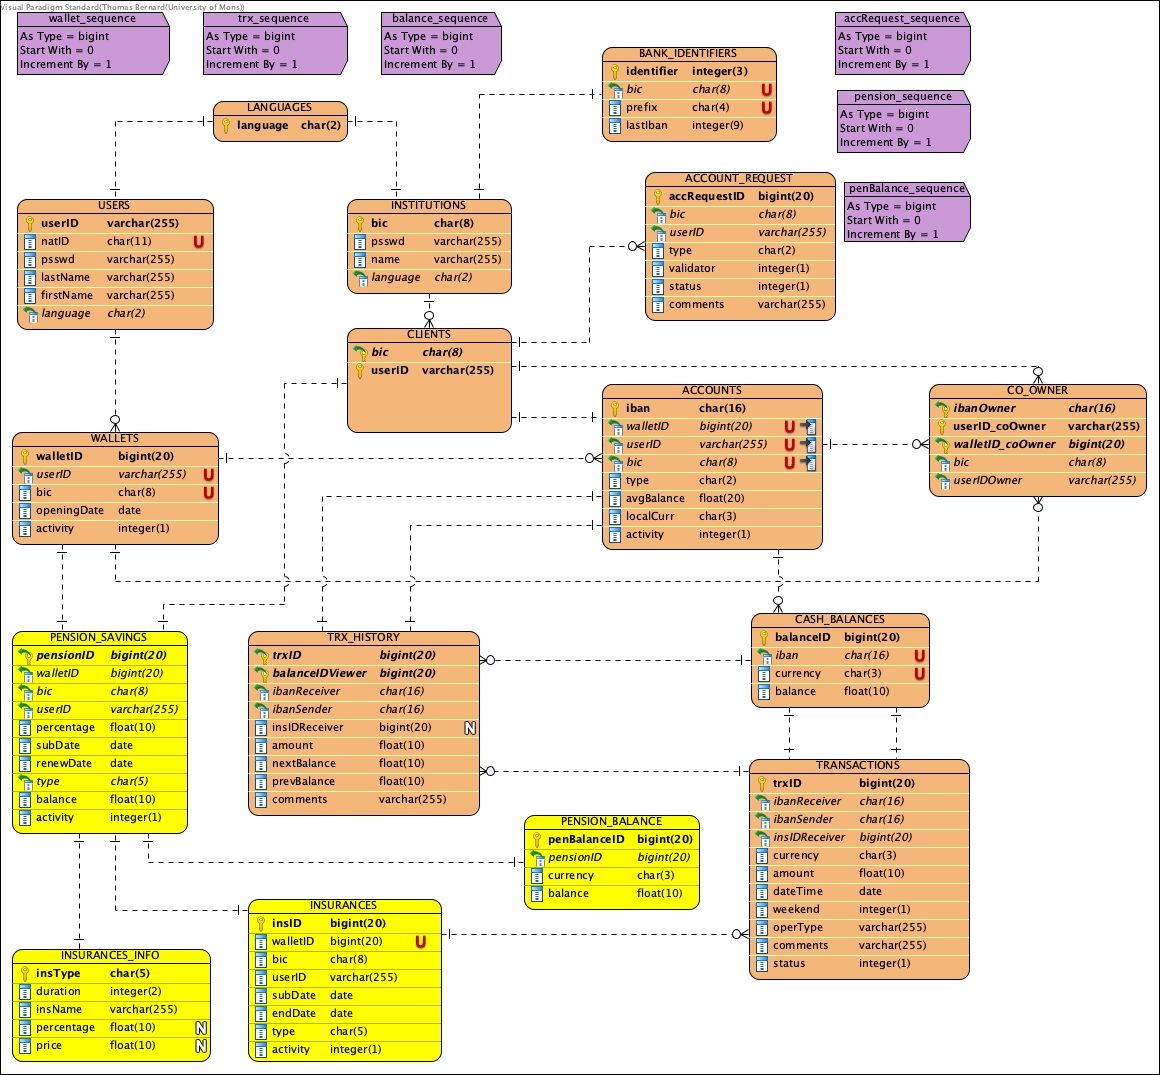
\includegraphics[scale=0.3]{ressources/finalDb.jpg}
			\caption{Diagramme d'entité-relation de la base de données.}
		\end{figure}

\newpage

\subsection{API}

\paragraph{Choix du framework }
Lors de l'implémentation de l'API nous avons eu 2 choix qui se sont offerts à nous : Faire l'API à partir de rien ou bien utiliser un framework.
Suite à la présentation du framework Spring par Jeremy Dubrulle nous avons décidés d'opter pour celui-ci car il nous permettait de nous familiariser avec
le concept d'API ainsi qu'avec son fonctionnement en enlevant quelque peu ce côté obscur que ce concept peut avoir.

\medskip

Spring porpose de nombreuses dependances notamment Spring Data Jpa dont nous avons parlé dans la section liée à la BDD, mais également Lombok dont nous nous sommes servis afin d'auto générer
les getter, setter et constructeurs de classes. 

\paragraph{Architecture d'implémentation de Spring}

Une API réalisée avec le framework Spring possède une architecture spécifique sous la forme de 3 couches qui communiquent les unes avec les autres :

\medskip
\begin{enumerate}
	\item\textbf{Les Controllers : } Il s'agit de la couche qui se charge de la communication avec le côté client. En effet celle-ci définit les URI vers lesquels les requêtes doivent être
		envoyées. Cette couche se charge également de renvoyer les données du côté client. C'est une couche de communication entre le client et le serveur. Le controller permet de définir
		des méthodes qui interprêtent les requêtes reçues et appellent les méthodes adéquates dans la couche suivante.
	\item\textbf{Les Services : } Il s'agit de la couche logique de l'API celle qui traite les informations, qu'elles proviennent des controllers ou bien des repositories qui envoient les données
		provenant de la BDD. Les services effectuent les actions demandées par les controllers et renvoie les données ou des erreurs dans le cas où une requête serait inadéquate ou que son contenu 
		serait introuvable.
	\item\textbf{Les Repositories : } Il s'agit de la couche qui se charge de la communication avce la BDD. Un Repository est une interface qui implémente des méthods qui incarnent elles-mêmes
		des requêtes en direction de la BDD. Les requêtes leurs sont spécifiées à l'aide du \@Query qui les précède. Les repositories se content d'exécuter les requêtes mais ne vérifient pas qu'il
		s'agisse du contenu souhaité car c'est le rôle des services. Les seules erreurs que les repositories renvoient sont des erreurs liées à la BDD (mauavaise requête, non respect de contraintes).
\end{enumerate}

\paragraph{Gestion des entités}
Le framework Spring utilise des classes de typoe Entity afin de définir les tables représentées dans la BDD chaque table est représentée par une classe de type Entity. Au sein de ces classes sont
définies les différents colonnes ainsi que leurs types et les contraintes qui leurs sont apppliquées. Cet outil permet de faciler l'accès aux données ainsi que la communication entre les données
d'entités différentes.

\bigskip

\paragraph{Gestion des transactions/requêtes} 
Notre application permet d'effectuer des transactions entre deux comptes bancaires, de simuler un dépôt bancaire ou bien encore de financer une assurance (pas implémenté côté client pour cette
dernière) et ce que ce soit de manière immédiate ou bien planifiée dans le temps. Nous avons opté pour un Scheduler qui va contrôler tous les jours la BDD pour savoir s'il faut effectuer des 
transactions. Pour celà nous nous servons de la classe \textit{TrxScheduler}.

\medskip

Cette classe est une nouvelle fois utilisée pour gérer les requêtes de souscriptions aux produits financiers stockées dans la table \textit{ACCOUNT\_REQUEST} accessible depuis l'application
des institutions. Les institutions peuvent valider ces requêtes une fois validée le \textit{validator} est mis à jour dans la table et le scheduler peut exécuter la création du produit financier.


\bigskip

\subsection{Manquements et problèmes du serveur}
Suite à la refonte de la répartition des tâches et à la réduction du nombres d'étudiants travaillant sur le serveur de 2 à 1, certaines fonctionnalités sont absentes du serveur.

\medskip

	\begin{enumerate}
		\item\textbf{Système de notifications :} Le système de notifications n'est malheureusement pas présent et pas géré. Toutefois pour ce qui est de la création de produit
			financier. Il existe un système de demande de création implémenté et fonctionnant de manière asynchrone entre l'application client et l'application institution.
		\item\textbf{Sécurité : } Le serveur ainsi que les requêtes sont en protocole HTTP au lieu de HTTPS. Ugo devait se charger d'implémenter Spring Security afin de sécuriser nos requêtes
			et notre API malheureusement cette fonctionnalité manque à l'appel.
		\item\textbf{Tests unitaires : } Ugo avait également pour tâche d'effectuer les tests unitaires de l'API, la tâche a finalement été réattribuée vers Thomas mais trop tard pour faire 
			face au problème de communication entre les DATA JPA et l'instance en mémoire de BDD H2 servant aux tests. Afin d'effectuer les tests il aurait fallu changer totalement de framework
			ce qui était impossible à ce stade du projet.
		\item\textbf{Création des portfeuilles : } La création des portfeuilles n'est pas soumise à une approbation de l'institution, il s'agirait d'un fonctionnalité simple d'ajout mais coûteuse
			en temps car elle implique de gérer autrements certaines tables de la BDD.
	\end{enumerate}

\newpage
\end{document}

